\documentclass[12pt]{article}
\usepackage[a4paper, margin=1in]{geometry} 
\usepackage{graphicx} 
\usepackage{hyperref}
\usepackage{float}
\usepackage{multicol}
\usepackage{multirow}
\usepackage{amsmath}
\usepackage[ruled]{algorithm2e}
\usepackage{amssymb}
\usepackage[font=small, labelfont=bf]{caption}
\usepackage[table,xcdraw]{xcolor}

\title{Lecture Notes for \\ INF281 Basics of Bioinformatics Sequence Analysis}
\author{Takaya Saito}
\date{}

\begin{document}

\pagenumbering{arabic}
\setcounter{page}{63}

\makeatletter 
\renewcommand{\thefigure}{\arabic{section}.\arabic{figure}}
\renewcommand{\thetable}{\arabic{section}.\arabic{table}}
\makeatother

%
% Phylogenetic tree
%
\setcounter{section}{8}
\setcounter{figure}{0}
\setcounter{table}{0}
\section{Phylogenetic tree}
%\documentclass[12pt]{article}
%\usepackage[a4paper, margin=1in]{geometry} 
%\usepackage{graphicx} 
%\usepackage{hyperref}
%\usepackage{float}
%\usepackage{multicol}
%\usepackage{multirow}
%\usepackage{amsmath}
%\usepackage[font=small, labelfont=bf]{caption}
%
%\begin{document}

%
% Introduction to phylogenetic trees
%
\subsection{Introduction to phylogenetic trees}
A phylogenetic provides additional views on the analysis of multiple sequences.

%
% Elements of phylogenetic tree
%
\subsubsection*{Elements of phylogenetic tree}
\begin{itemize}
\item Terminal nodes: sequences, gruops of genes, species, operational taxonomic units
\item Internal nodes: hypothetical ancestral units
\item Edges: often represent distances
\end{itemize}

%
% Types of trees
%
\subsubsection*{Types of trees}
\begin{itemize}
\item Cladogram or phylogram
\item Bifurcating or multifurcating
\item Rooted or unrooted
\end{itemize}

\begin{figure}[H]
  \centering
      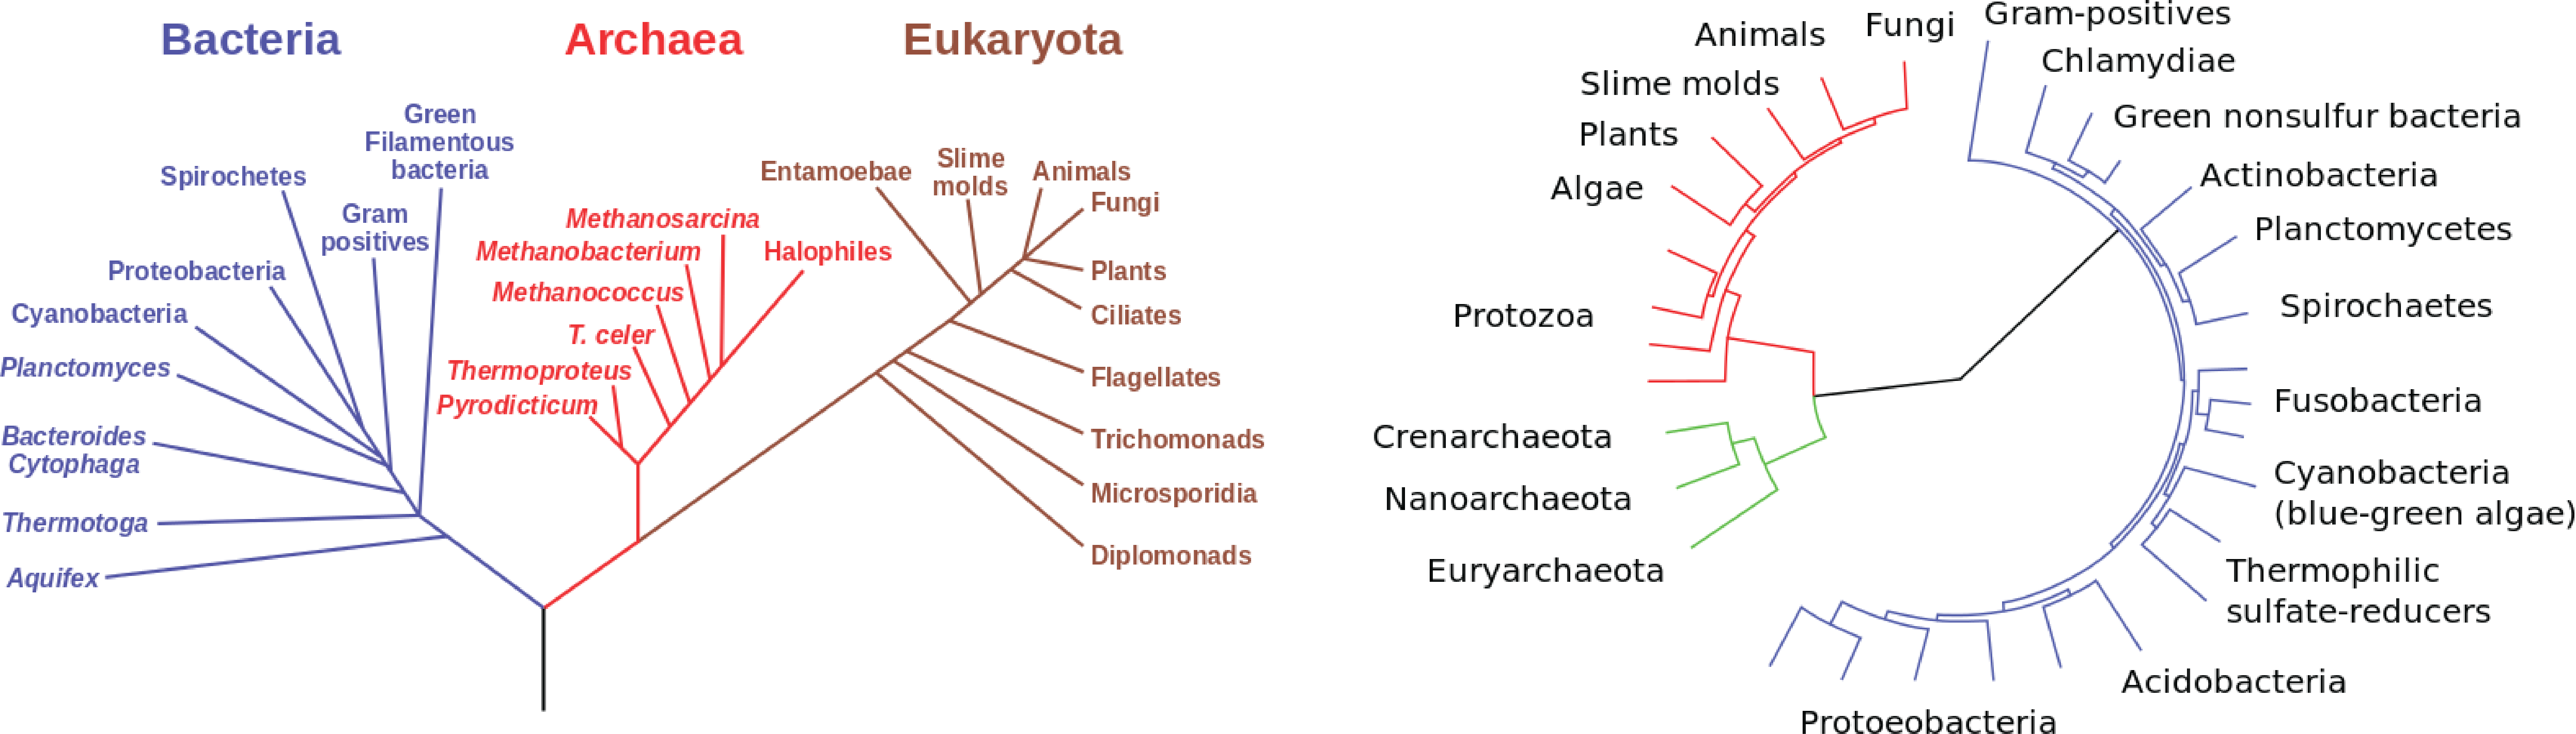
\includegraphics[width=0.75 \textwidth]{fig09/root_unroot_tree_example.png}
  \caption{Phylogenetic trees (sources: \href{https://commons.wikimedia.org/w/index.php?curid=9381199}{TimVickers, Wikimedia Commons}, \href{https://commons.wikimedia.org/w/index.php?curid=1201601}{NASA Astrobiology Institute, Wikimedia Commons}))}
\end{figure}

%
% Rooted and unrooted trees
%
\subsubsection*{Rooted and unrooted trees}
\begin{figure}[H]
  \centering
      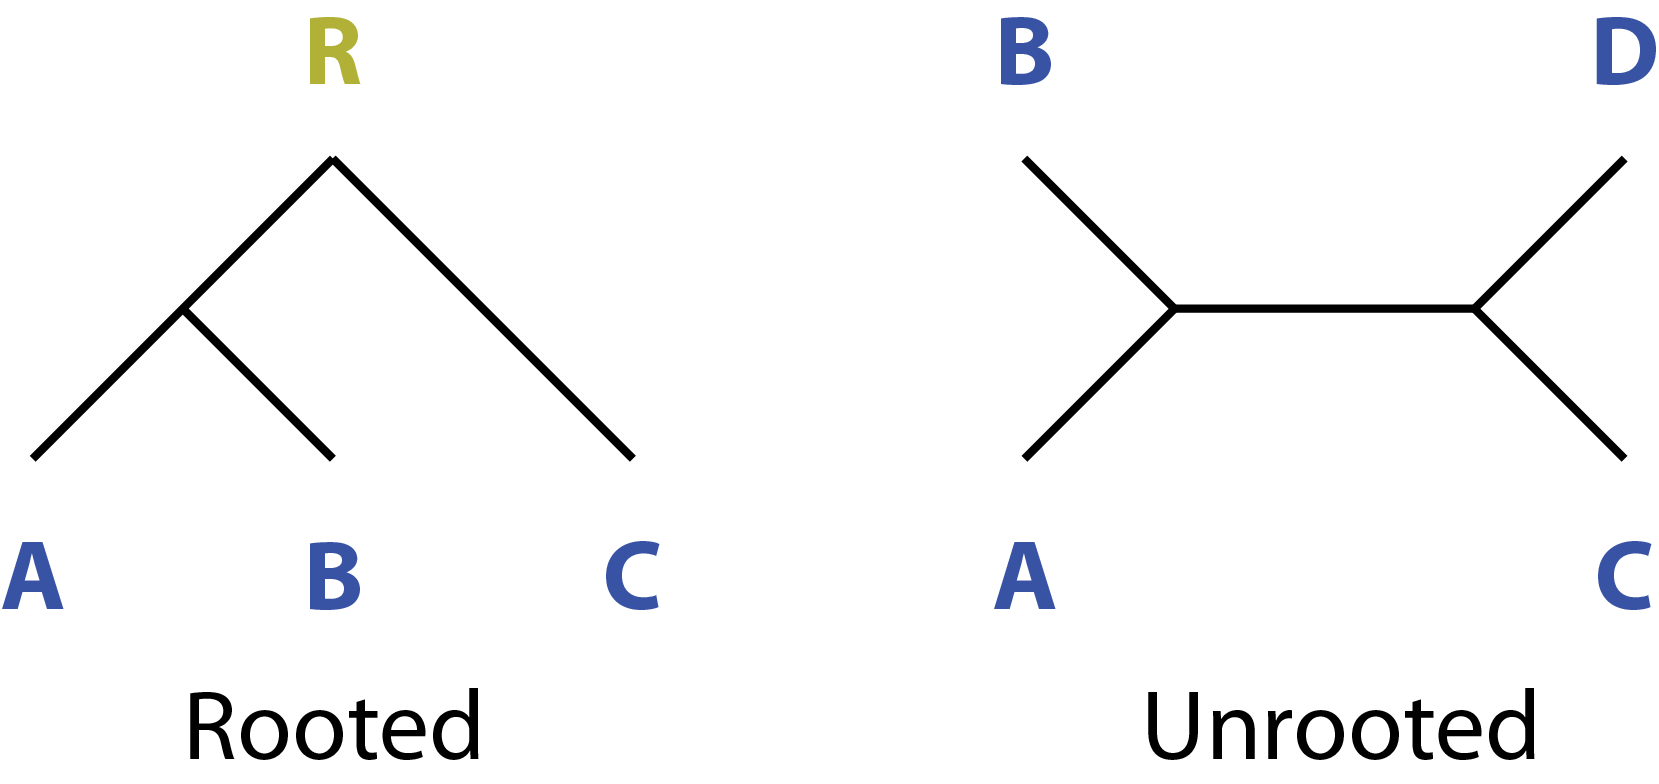
\includegraphics[width=0.35 \textwidth]{fig09/root_unroot_trees.png}
  \caption{A rooted tree with three nodes and an unrooted tree with four nodes}
\end{figure}

%
% Additive and ultrametric trees
%
\subsubsection*{Additive and ultrametric trees}
\begin{figure}[H]
  \centering
      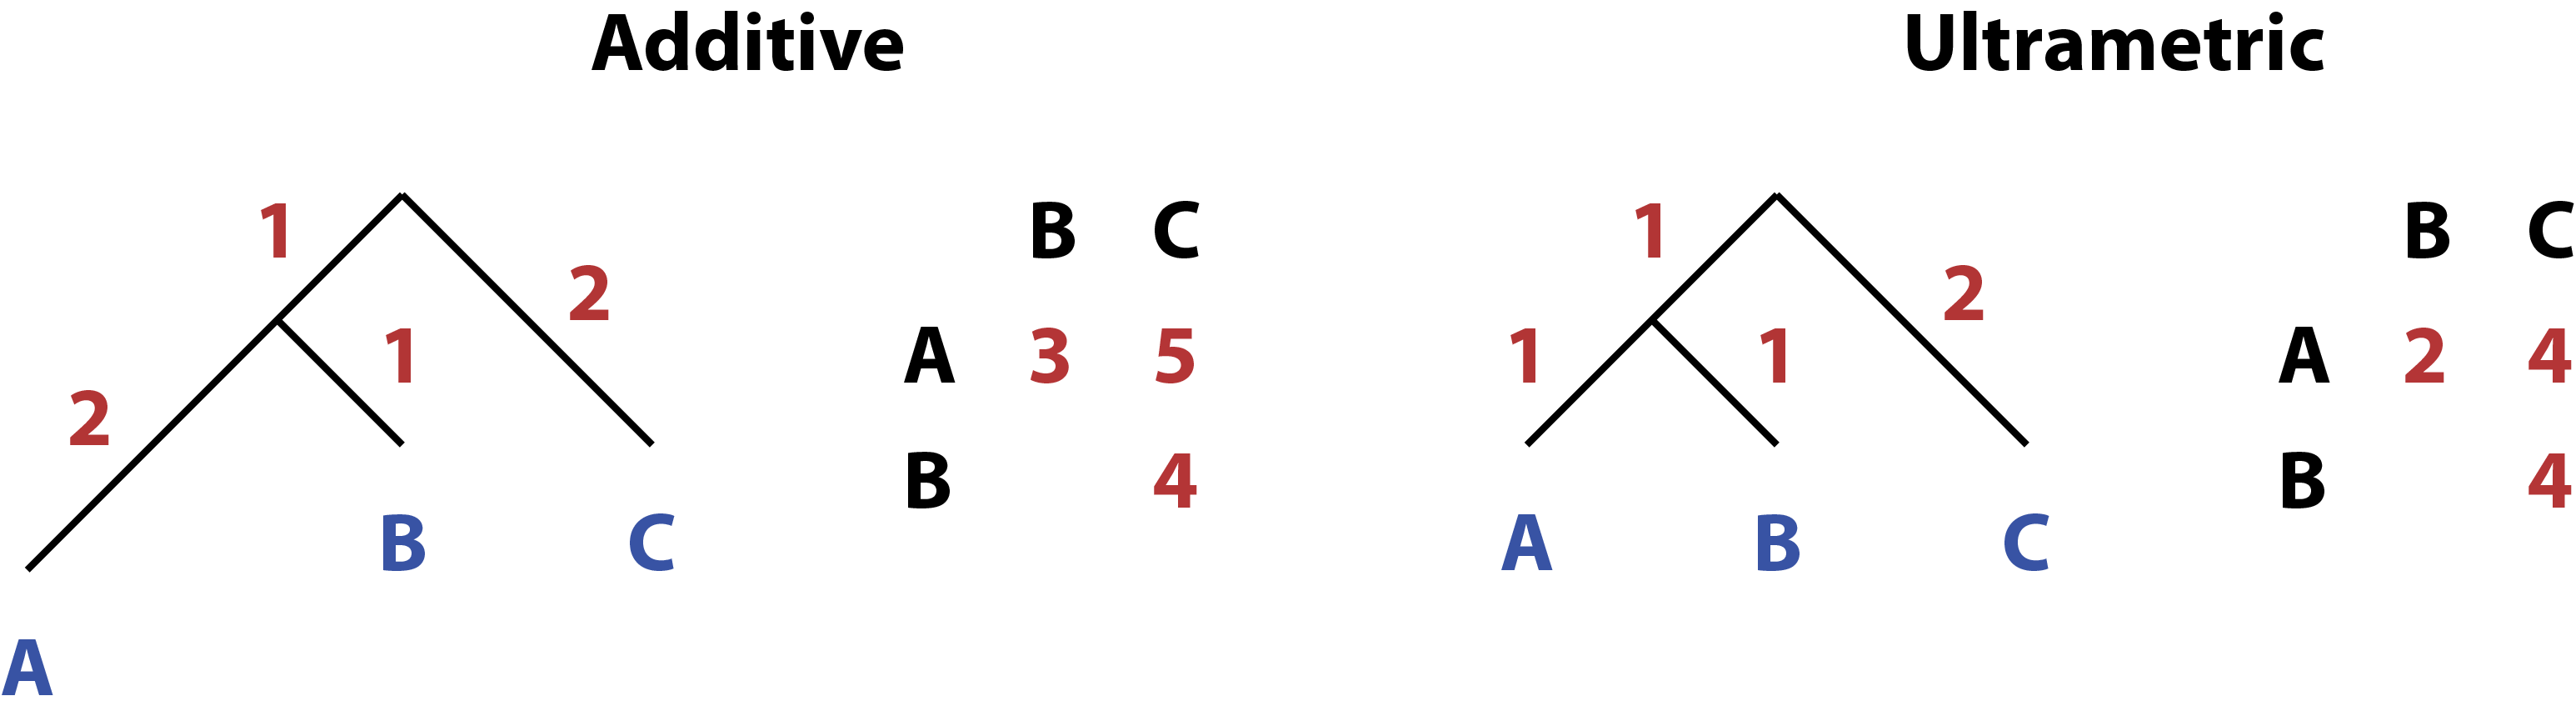
\includegraphics[width=0.6 \textwidth]{fig09/additive_ultrametric.png}
  \caption{Additive and ultrametric trees}
\end{figure}
An ultrrametic tree is a special version of additive tree. It assumes that the distances from two sequences to their common ancestor are always equal.

%
% Number of topologically different tree
%
\subsubsection*{Number of topologically different trees}
\begin{figure}[H]
  \centering
      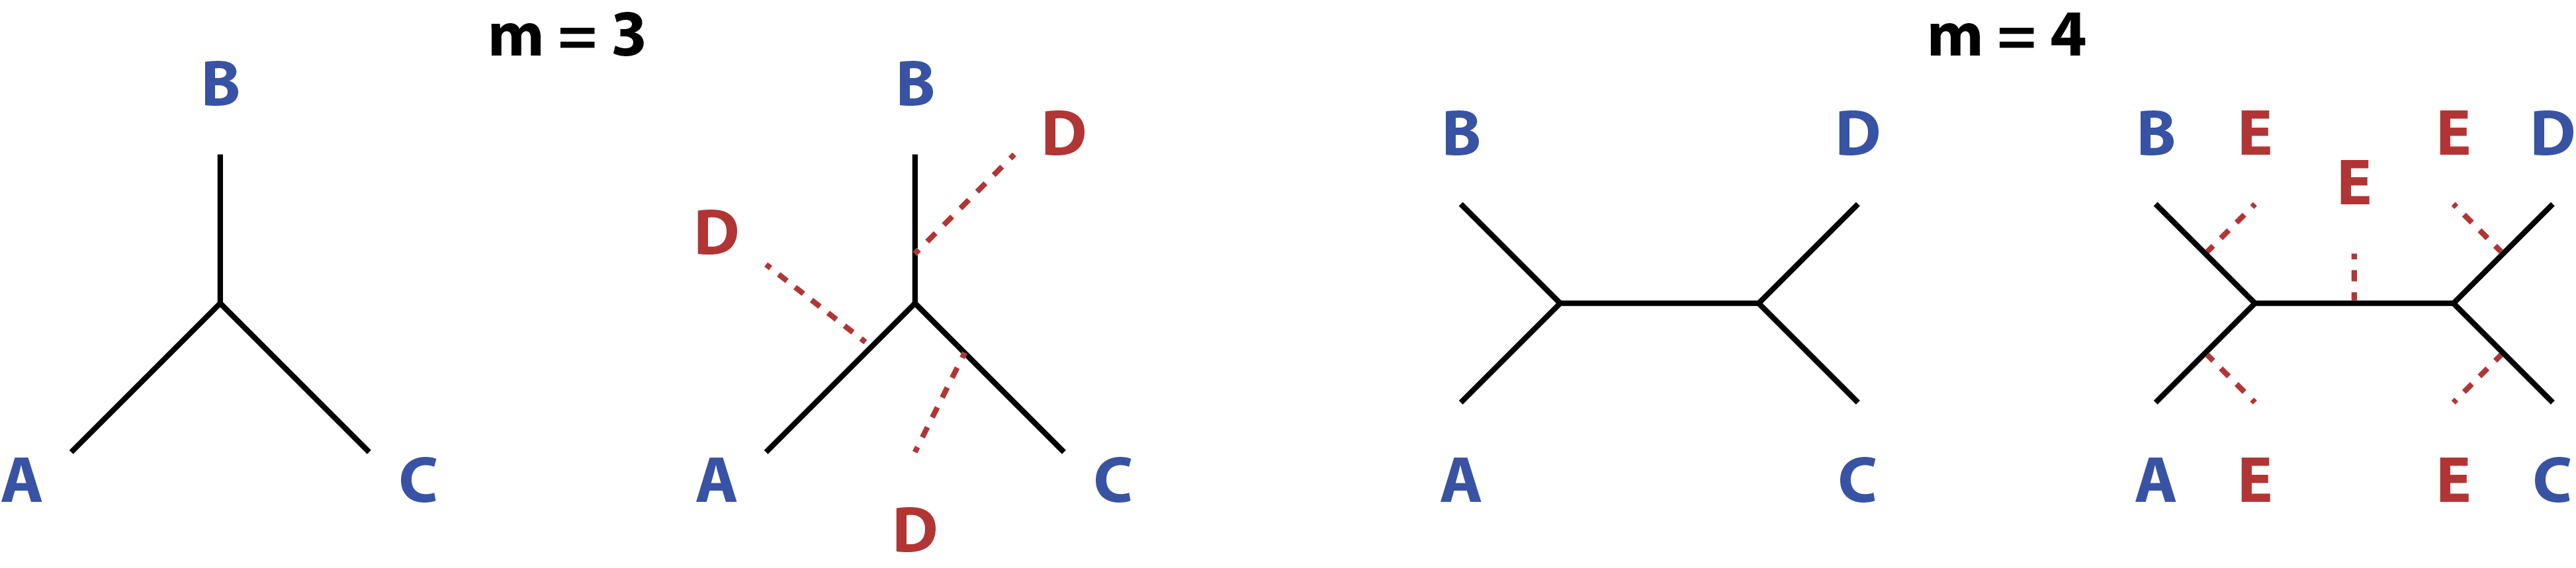
\includegraphics[width=0.7 \textwidth]{fig09/unroot_topology.png}
  \caption{Adding one external node to unrooted trees}
\end{figure}

The number of all possible topologically different unrooted trees $\mathrm{T_{unroot}}(m)$ can be obtained by the double factorial of $2m-5$.

\[
\mathrm{T_{unroot}}(m) = (2m - 5)!! \equiv \dfrac{(2m-5)!}{2^{m-3}(m-3)!}
\]
\medskip

\noindent
$\mathrm{T_{root}}(m)$ can be calculated from $\mathrm{T_{unroot}}(m)$. 

\[
\mathrm{T_{root}}(m) = (m-1) \times \mathrm{T_{unroot}}(m)
\]

%
% Example of the number of unrooted tree
%
\subsubsection*{Example of the number of unrooted trees}
What is the number of all possible topologically different unrooted trees when m = 7?

\[
\mathrm{T_{unroot}}(7) = (2 \times 7 - 5)!! = 9!! =1 \times 3 \times 5 \times 7 \times9 = 945
\]

or

\[
\mathrm{T_{unroot}}(7) = \dfrac{(2 \times 7 - 5)!}{2^{7-3}(7-3)!} = \dfrac{9!}{2^{4}(4)!} = 945
\]

%
% Exercise \thesection.1
%
\subsubsection*{Exercise \thesection.1}
\begin{enumerate}
\item Calculate the number of all possible topologically different unrooted trees when m = 5.
\medskip 

\item Construct an additive rooted tree for the distance matrix below. Estimate the edge values by trial and error.
\end{enumerate}

\begin{table}[H]
\centering
\begin{tabular}{|l|l|l|}
\hline
  & B & C \\ \hline
A & 4 & 7 \\ \hline
B &   & 5 \\ \hline
\end{tabular}
\end{table}

\bigskip 

%\end{document}

%\documentclass[12pt]{article}
%\usepackage[a4paper, margin=1in]{geometry} 
%\usepackage{graphicx} 
%\usepackage{hyperref}
%\usepackage{float}
%\usepackage{multicol}
%\usepackage{multirow}
%\usepackage{amsmath}
%\usepackage[font=small, labelfont=bf]{caption}
%
%\begin{document}

%
% Tree reconstruction methods
%
\subsection{Tree reconstruction methods}
A number of methods have been proposed to reconstruct a phylogenetic tree.

%
% Two types of reconstruction methods
%
\subsubsection*{Two types of reconstruction methods}
\begin{itemize}
\item Distance-based methods
\item Character-based methods
\end{itemize}

%
% Distance-based methods
%
\subsubsection*{Distance-based methods}
A distance is a positive value with larger values indicating that two sequences are separated further. 

\begin{itemize}
\item PGMA (pair-group method using arithmetic mean)
\item Neighbor-joining  (NJ)
\end{itemize}

%
% Character-based methods
%
\subsubsection*{Character-based methods}
Character based methods rely on characters (amino acid/nucleotide letters) to reconstruct a tree.

\begin{itemize}
\item Maximum parsimony
\item Maximum likelihood
\end{itemize}

% Evaluation of reconstructed tree
%
\subsubsection*{Evaluation of reconstructed trees}
Bootstrapping is one of the methods to test the robustness of a reconstruct tree by adding noises and comparing the results.
\begin{enumerate}
\item Randomly generate a pseudo MAS from the original MSA
\item Reconstruct a tree
\item Repeat the process
\item Compare the trees
\end{enumerate}

\bigskip 

%\end{document}

%\documentclass[12pt]{article}
%\usepackage[a4paper, margin=1in]{geometry} 
%\usepackage{graphicx} 
%\usepackage{hyperref}
%\usepackage{float}
%\usepackage{multicol}
%\usepackage{multirow}
%\usepackage{amsmath}
%\usepackage[font=small, labelfont=bf]{caption}
%
%\begin{document}

%
% Distance-based methods
%
\subsection{Distance-based methods}
PGMA (pair-group method using arithmetic mean) and neighbor-joining are two popular distance-based methods to reconstruct a phylogenetic tree.

%
%  UPGMA
%
\subsubsection*{UPGMA}
UPGMA is an unweighted version of PGMA. It requires the evolutionary rate should be constant (ultrametric). Pairwise distances need to be pre-calculated, for instance, by DP.

\begin{itemize}
\item $w$: A new node
\item $u$, $\upsilon$: Child nodes of $w$
\item $m_{A}$ The number of original sequences in subtree $A$
\item $D_{A,B}$: Distance between sequences/subtrees $A$ and $B$
\end{itemize}

\[
D_{w,x}=\dfrac{m_{u}D_{u,x} + m_{\upsilon}D_{\upsilon,x}}{m_{u} + m_{\upsilon}}
\]

%
% Example of UPGMA
%
\subsubsection*{Example of UPGMA}
Reconstruct a phylogenetic tree from the pre-calculated distances below.

\begin{table}[H]
\centering
\begin{tabular}{|l|l|l|l|}
\hline
  & B & C & D \\ \hline
A & 4 & 2 & 5 \\ \hline
B &   & 4 & 8 \\ \hline
C &   &   & 5 \\ \hline
\end{tabular}
\end{table}

\noindent
\textbf{Step 1a}.
Find a pair with the closest distance
\begin{figure}[H]
  \centering
      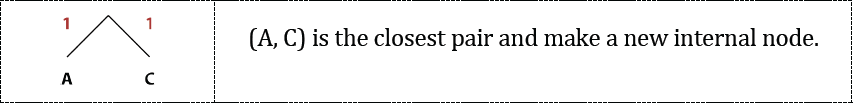
\includegraphics[width=0.9 \textwidth]{fig09/upgma_1.png}
\end{figure}

\noindent
\textbf{Step 1b}.
Recalculate the distances
\[
d_{B,(AC)}=\dfrac{d_{B,A} + d_{B,C}}{2} = 4, \quad d_{D,(AC)}=\dfrac{d_{D,A} + d_{D,C}}{2} = 5
\]

\noindent
\textbf{Step 1c}.
Update the distance matrix with a new node (AC)
\begin{table}[H]
\centering
\begin{tabular}{|l|l|l|}
\hline
     & B & D \\ \hline
(AC) & 4 & 5 \\ \hline
B    &   & 8 \\ \hline
\end{tabular}
\end{table}

\noindent
\textbf{Step 2a}.
Find a pair with the closest distance
\begin{figure}[H]
  \centering
      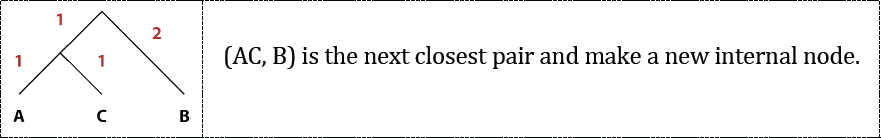
\includegraphics[width=0.9 \textwidth]{fig09/upgma_2.png}
\end{figure}

\noindent
\textbf{Step 2b}.
Recalculate the distance
\[
d_{((AC)B),D}=\dfrac{2 \times d_{(AC),D} + d_{B,D}}{3} = 6
\]

\noindent
\textbf{Step 2c}.
Update the distance matrix with a new node ((AC)B)
\begin{table}[H]
\centering
\begin{tabular}{|l|l|}
\hline
        & D \\ \hline
((AC)B) & 6 \\ \hline
\end{tabular}
\end{table}

\noindent
\textbf{Step 3}.
Complete the tree
\begin{figure}[H]
  \centering
      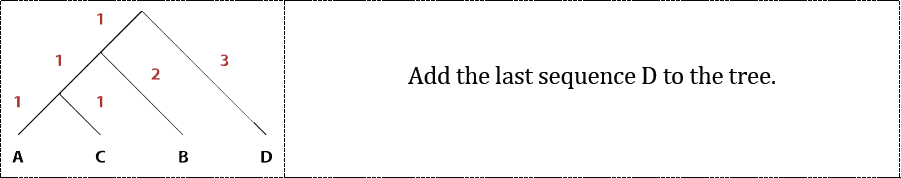
\includegraphics[width=0.9 \textwidth]{fig09/upgma_3.png}
\end{figure}

%
% Evaluation on how well fitted to the original distances
%
\subsubsection*{Evaluation on how well fitted to the original distances}
Several criteria are available to find the best-fitted tree for a given distance matrix, such as the Cavalli-Sforza and Edwards criterion:

\[
\sum_{i,j}{}(M_{i,j} - d_{i,j})^2
\]

where $M_{i,j}$ and $d_{i,j}$ are respectively the original and the calcualted pairwise distances.

%
% Example of the Cavalli-Sforza and Edwards criterion 
%
\subsubsection*{Example of the Cavalli-Sforza and Edwards criterion}

\begin{table}[H]
\centering
\begin{tabular}{lllllllll}
\multicolumn{4}{l}{Original}                                                                       &                       & \multicolumn{4}{l}{Reconstructed}                                                                 \\ \cline{1-4} \cline{6-9} 
\multicolumn{1}{|l|}{}  & \multicolumn{1}{l|}{B} & \multicolumn{1}{l|}{C} & \multicolumn{1}{l|}{D} & \multicolumn{1}{l|}{} & \multicolumn{1}{l|}{}  & \multicolumn{1}{l|}{B} & \multicolumn{1}{l|}{C} & \multicolumn{1}{l|}{D} \\ \cline{1-4} \cline{6-9} 
\multicolumn{1}{|l|}{A} & \multicolumn{1}{l|}{4} & \multicolumn{1}{l|}{2} & \multicolumn{1}{l|}{5} & \multicolumn{1}{l|}{} & \multicolumn{1}{l|}{A} & \multicolumn{1}{l|}{4} & \multicolumn{1}{l|}{2} & \multicolumn{1}{l|}{6} \\ \cline{1-4} \cline{6-9} 
\multicolumn{1}{|l|}{B} & \multicolumn{1}{l|}{}  & \multicolumn{1}{l|}{4} & \multicolumn{1}{l|}{8} & \multicolumn{1}{l|}{} & \multicolumn{1}{l|}{B} & \multicolumn{1}{l|}{}  & \multicolumn{1}{l|}{4} & \multicolumn{1}{l|}{6} \\ \cline{1-4} \cline{6-9} 
\multicolumn{1}{|l|}{C} & \multicolumn{1}{l|}{}  & \multicolumn{1}{l|}{}  & \multicolumn{1}{l|}{5} & \multicolumn{1}{l|}{} & \multicolumn{1}{l|}{C} & \multicolumn{1}{l|}{}  & \multicolumn{1}{l|}{}  & \multicolumn{1}{l|}{6} \\ \cline{1-4} \cline{6-9} 
\end{tabular}
\end{table}

\[
\sum_{i,j}{}(M_{i,j} - d_{i,j})^2 = 2((5-6)^2 + (8-6)^2 + (5-6)^2) =12
\]

%
% WPGMA
%
\subsubsection*{WPGMA}
WPGMA is a weighted version of PGMA.

\[
D_{w,x}=\dfrac{D_{u,x} + D_{\upsilon,x}}{2}
\]

%
% Neighbor-joining (NJ) method
%
\subsubsection*{Neighbor-joining (NJ) method}
It stats with the initial tree and then select two seqences which results in the smallest sum of edge lengths. It continues until there are no sequences to join. Unlike UPGMA, it does not require a constant evolutionary rate.

\begin{figure}[H]
  \centering
      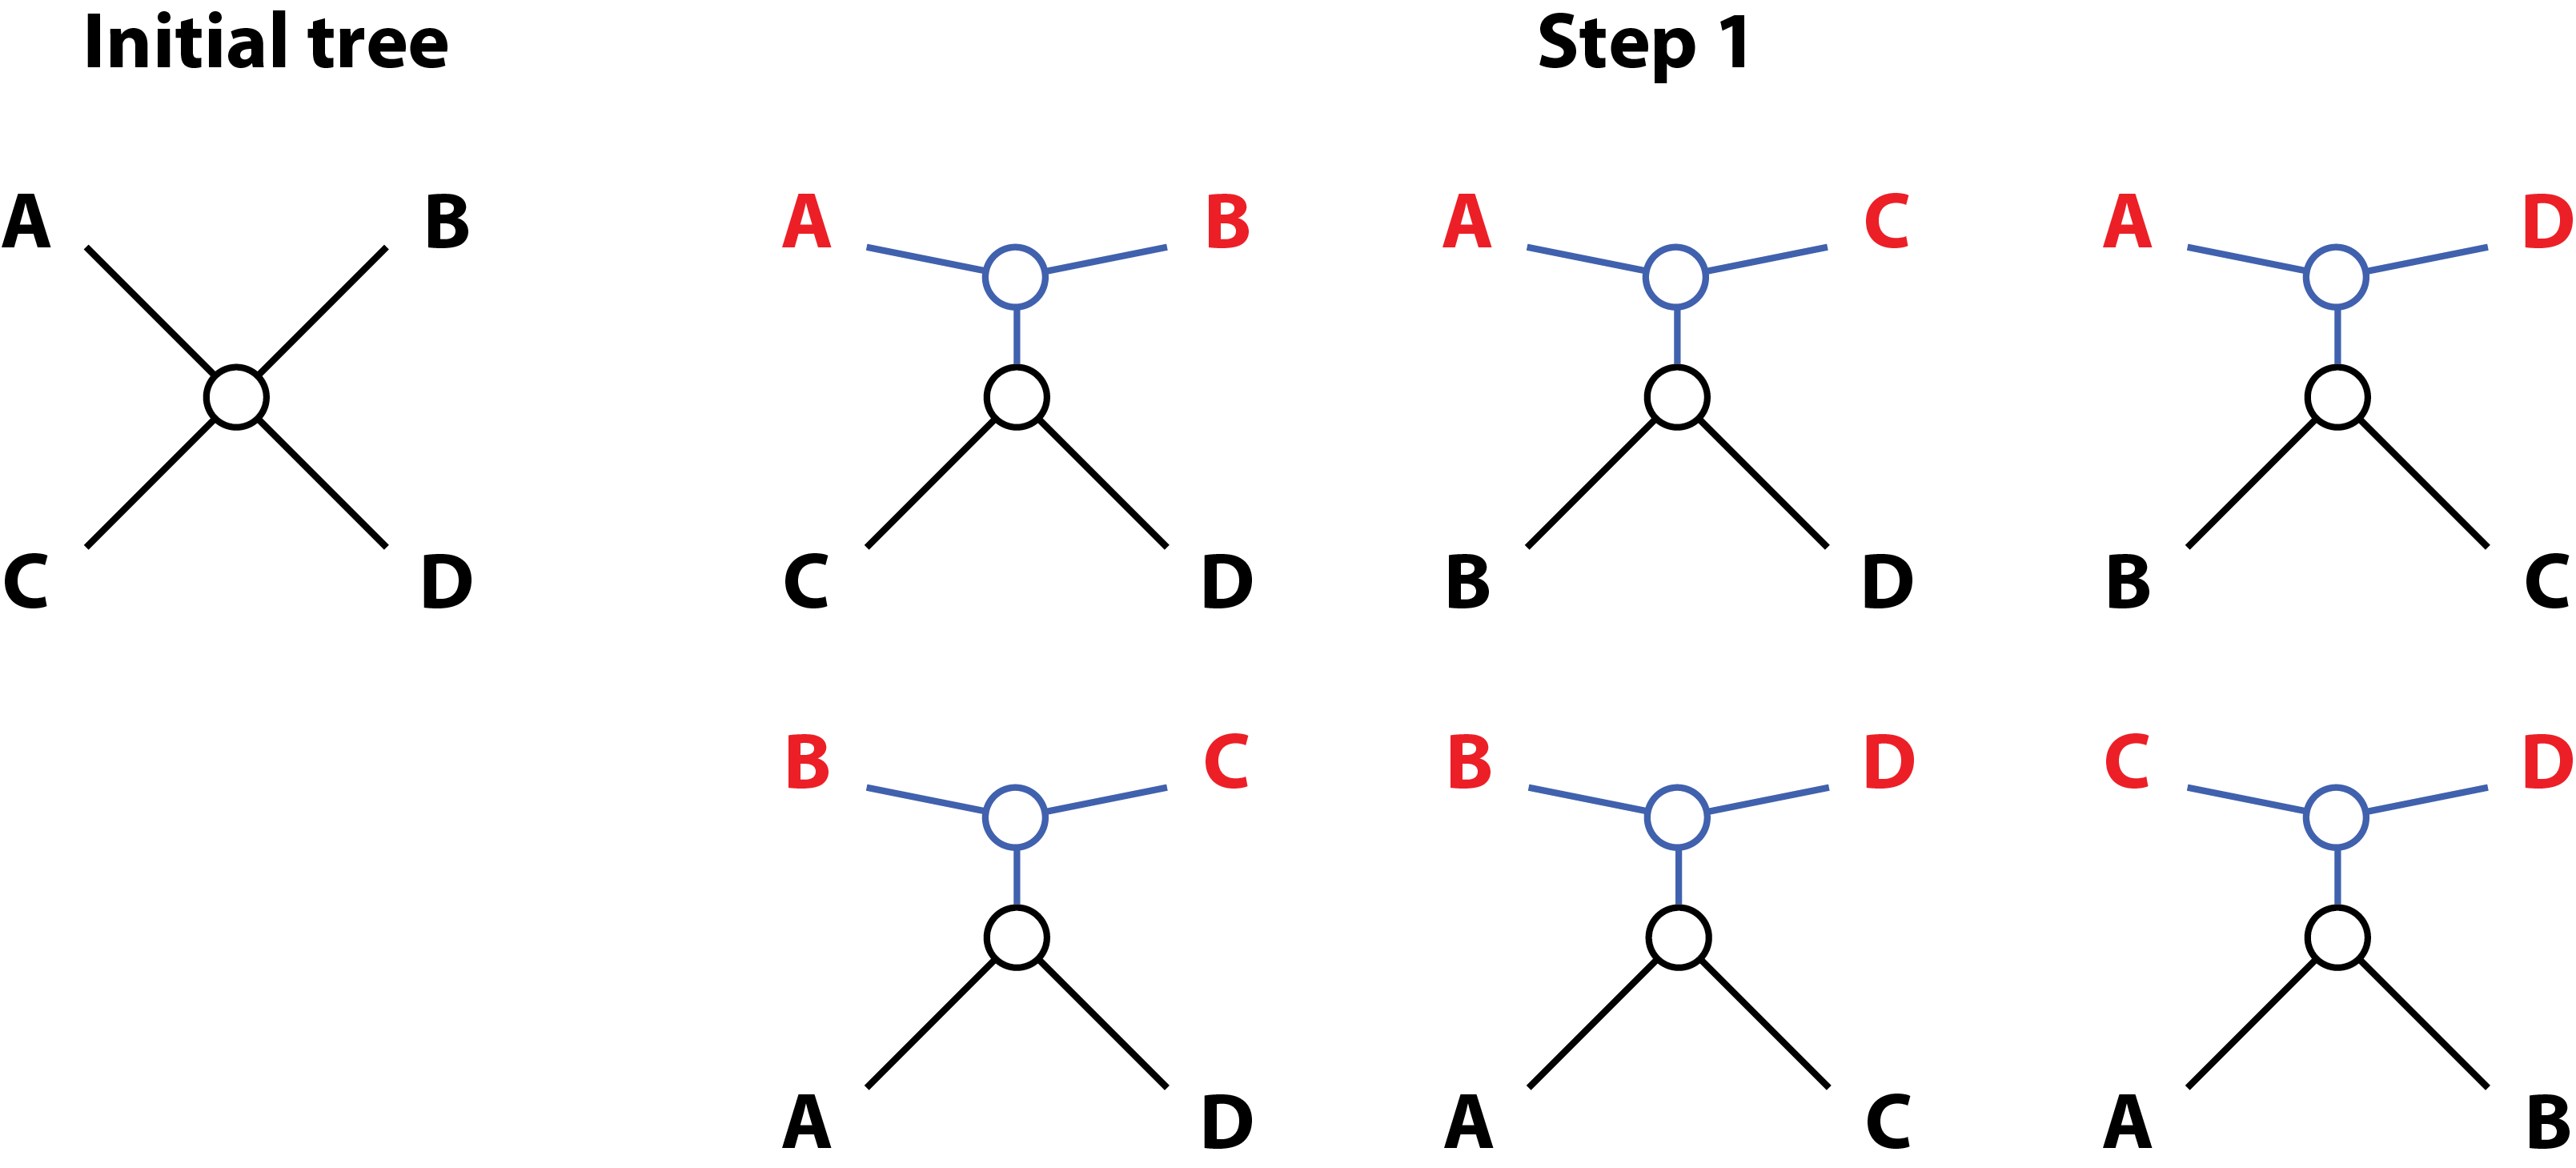
\includegraphics[width=0.75 \textwidth]{fig09/neighbor_joining.png}
  \caption{All possible combinations of adding one node the four sequences}
\end{figure}

%
% Exercise \thesection.2
%
\subsubsection*{Exercise \thesection.2}
\begin{enumerate}
\item Reconstruct a phylogenetic tree by using UPGMA and the following pre-calculated distances.
\begin{table}[H]
\centering
\begin{tabular}{|l|l|l|}
\hline
     & B & C \\ \hline
A  & 2 & 3 \\ \hline
B   &   & 5 \\ \hline
\end{tabular}
\end{table}

\item Create the distance matrix of the reconstructed tree. 
\begin{table}[H]
\centering
\begin{tabular}{|l|l|l|}
\hline
     & B & C \\ \hline
A  &  &  \\ \hline
B   &   &  \\ \hline
\end{tabular}
\end{table}

\item Calculated the Cavalli-Sforza and Edwards criterion.

\end{enumerate}

\bigskip 

%\end{document}

%\documentclass[12pt]{article}
%\usepackage[a4paper, margin=1in]{geometry} 
%\usepackage{graphicx} 
%\usepackage{hyperref}
%\usepackage{float}
%\usepackage{multicol}
%\usepackage{multirow}
%\usepackage{amsmath}
%\usepackage[ruled]{algorithm2e}
%\usepackage[font=small, labelfont=bf]{caption}
%
%\begin{document}

%
% Maximum parsimony
%
\subsection{Maximum parsimony}
Maximum parsimony is a character-based method to reconstruct a phylogenetic tree. 

%
%  Definition of parsimony
%
\subsubsection*{Definition of parsimony}
\begin{figure}[H]
  \centering
      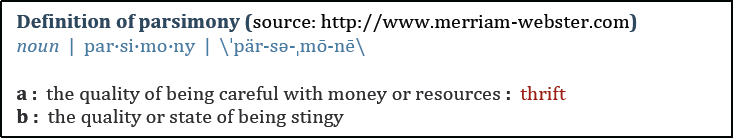
\includegraphics[width=0.7 \textwidth]{fig09/parsimony.png}
\end{figure}

%
%  Tree search method of maximum parsimony 
%
\subsubsection*{Tree search method of maximum parsimony}
The maximum parsimony method uses a tree search to find the tree with the minimum number of mutations. \\

\begin{algorithm}[H]    
  \BlankLine
  Construct an MSA;
  \BlankLine
    
  \ForEach{column $c$ $\in$ MSA}{
    \ForEach{tree $t$ $\in$ all possible topologically different trees}{
      Count the number of union operations in $c$ for tree $t$;
    }
    Add one point to the tree with the minimum union operations;
  }
  
  \BlankLine
  Report the tree with the maximum point;
   \BlankLine
    
  \SetAlgoRefName{\thesection.1}
  \caption{Maximum parsimony with the minimum union operations}

\end{algorithm}

%
%  Count the number of union operations
%
\subsubsection*{Count the number of union operations}
Either intersection or union operation is performed for each internal node.

\begin{itemize}
\item $s_i=s_j \cap s_k$ \quad If there is at least one element in $s_j$ and $s_k$
\item $s_i=s_j \cup s_k$ \quad Otherwise
\end{itemize}

%
% Example of counting the number of union operations
%
\subsubsection*{Example of counting the number of union operations}
Count the number of union operations for the first and the second columns.

\begin{figure}[H]
  \centering
      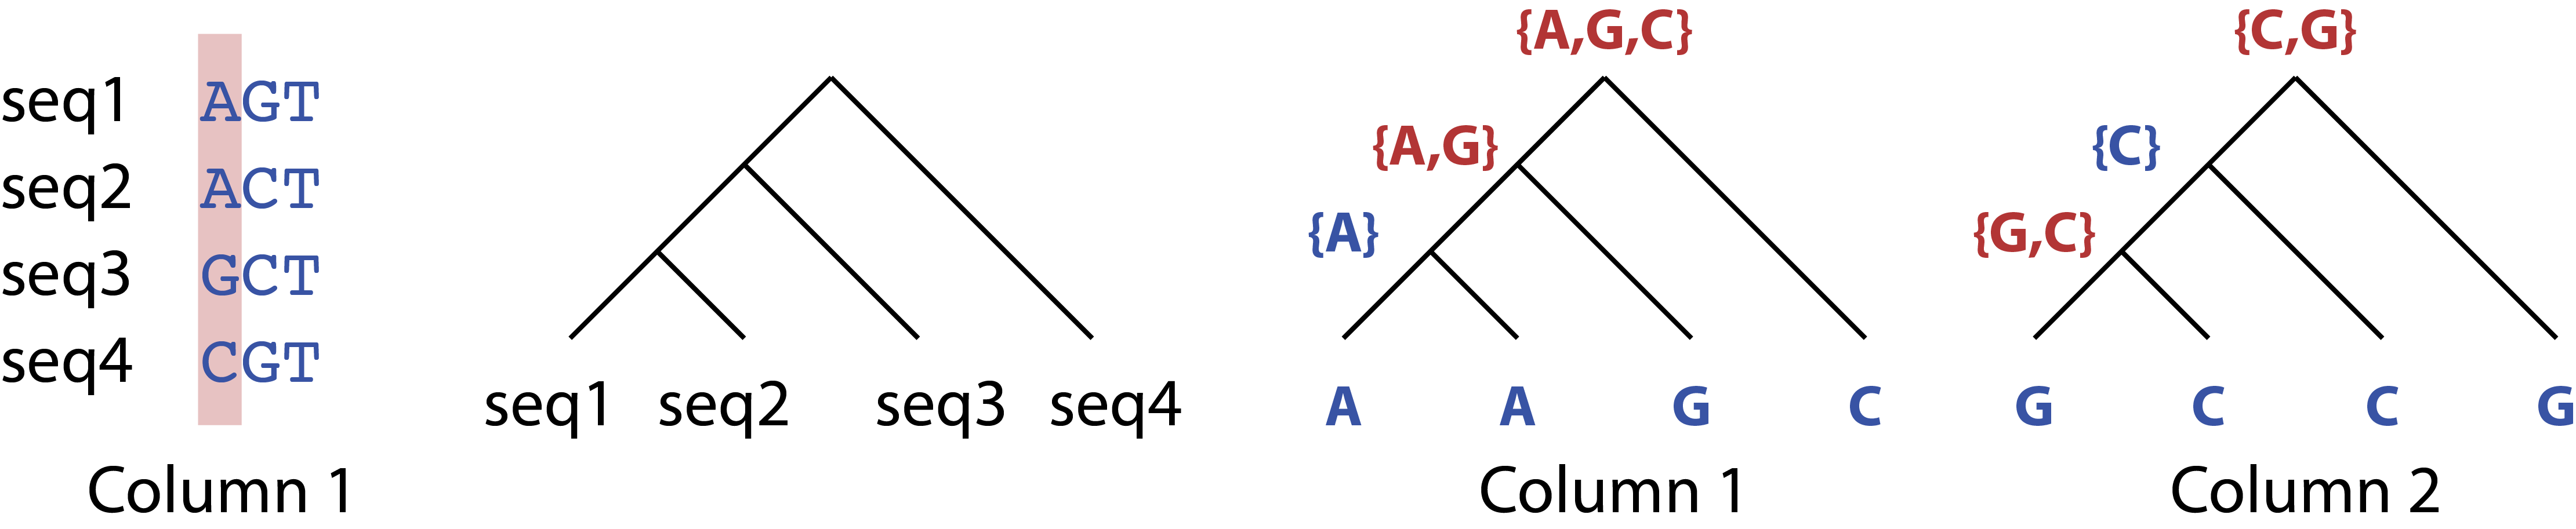
\includegraphics[width=0.8 \textwidth]{fig09/union_operations.png}
\end{figure}

\noindent
\textbf{Column 1}
\begin{itemize}
\item $A \cap A \rightarrow \{A\}$ 
\item $\{A\} \cup G \rightarrow \{A, G\}$ 
\item $\{A, G\} \cup C \rightarrow \{A, G, C\}$
\end{itemize}

\# of union operations: 2

\bigskip 

\noindent
\textbf{Column 2}
\begin{itemize}
\item $G \cup C \rightarrow \{G, C\}$ 
\item $\{G, C\} \cap C \rightarrow \{C\}$ 
\item $\{C\} \cup G \rightarrow \{C, G\}$
\end{itemize}

\# of union operations: 2

%
% Exercise \thesection.3
%
\subsubsection*{Exercise \thesection.3}
\begin{enumerate}
\item What is the number of union operations for the third column?
\begin{figure}[H]
  \centering
      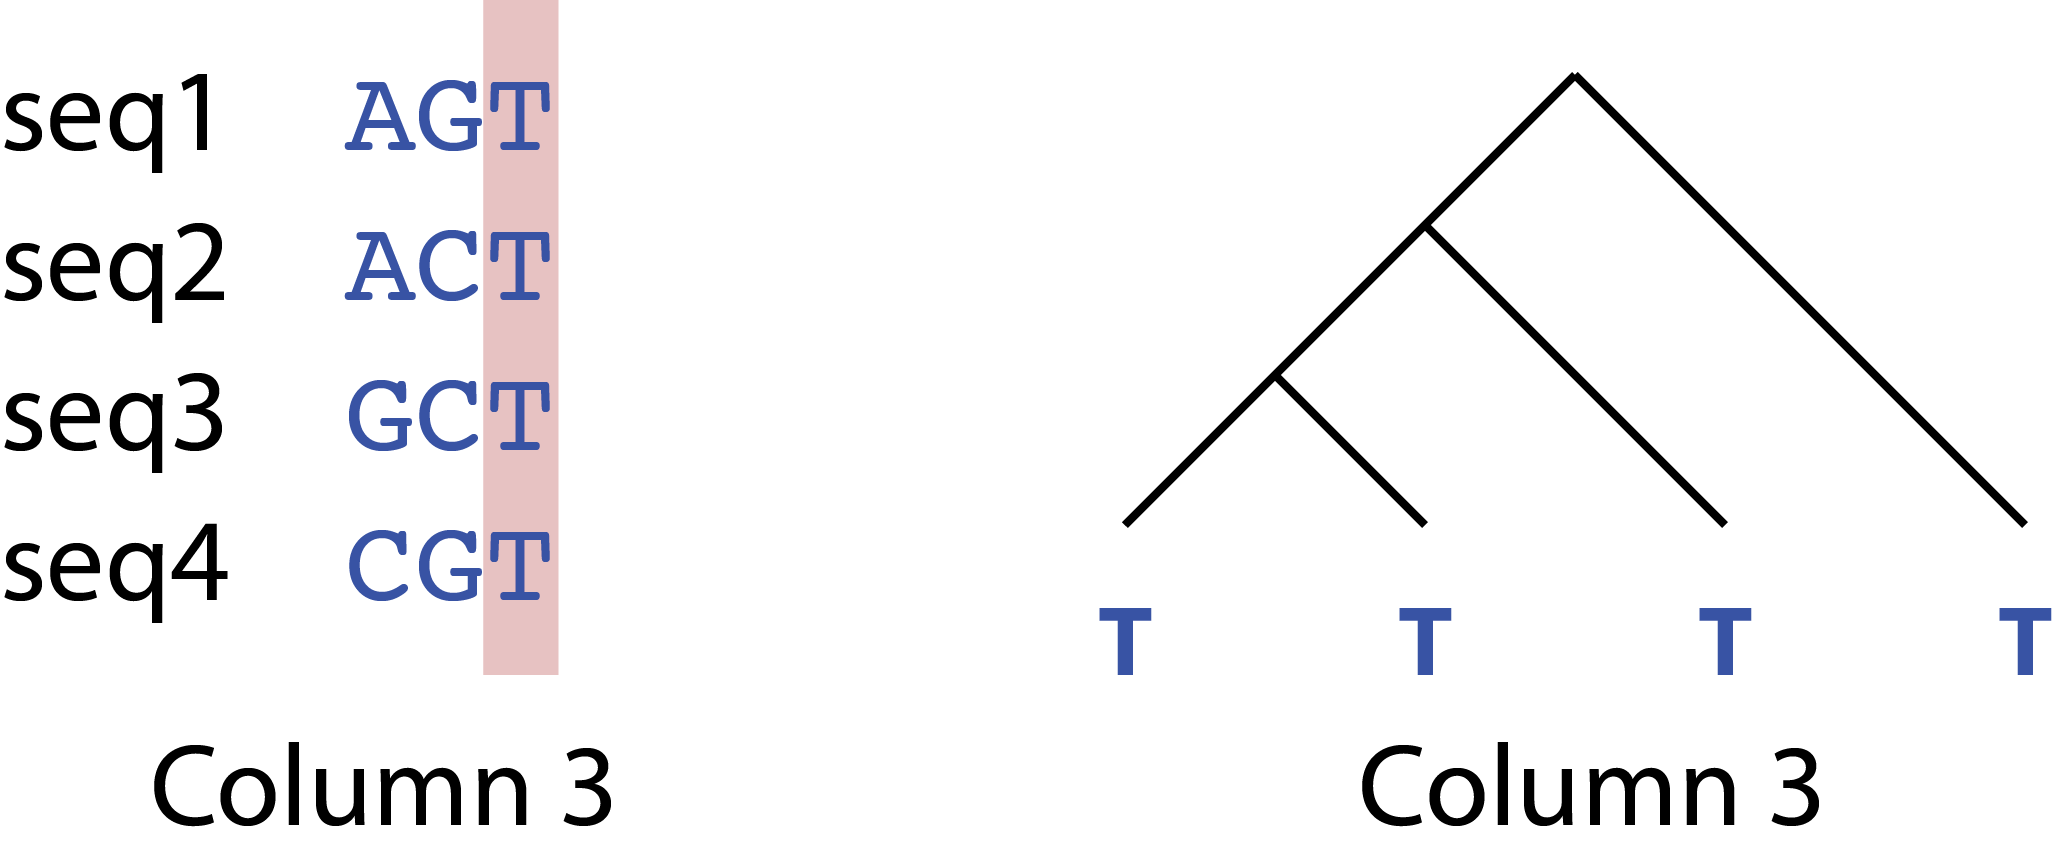
\includegraphics[width=0.4 \textwidth]{fig09/mp_exercise_1.png}
\end{figure}

\item What is the number of union operations for each column?
\begin{figure}[H]
  \centering
      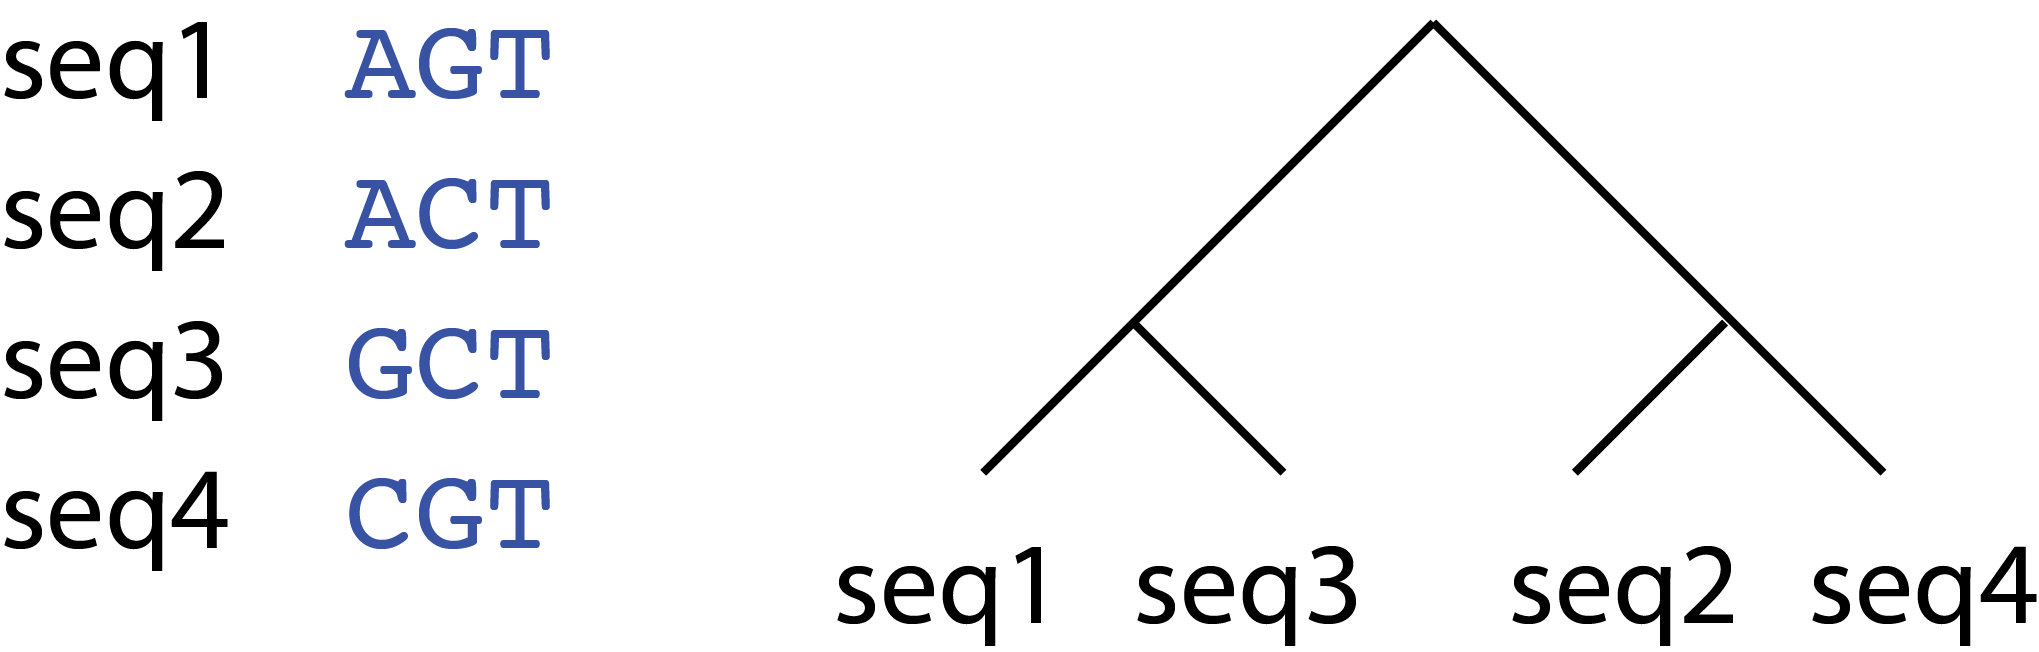
\includegraphics[width=0.4 \textwidth]{fig09/mp_exercise_2.png}
\end{figure}

\begin{itemize}
\item Column 1:
\item Column 2:
\item Column 3:
\end{itemize}

\end{enumerate}

\bigskip 

%\end{document}

%\documentclass[12pt]{article}
%\usepackage[a4paper, margin=1in]{geometry} 
%\usepackage{graphicx} 
%\usepackage{hyperref}
%\usepackage{float}
%\usepackage{multicol}
%\usepackage{multirow}
%\usepackage{amsmath}
%\usepackage[ruled]{algorithm2e}
%\usepackage[font=small, labelfont=bf]{caption}
%
%\begin{document}

%
% Maximum likelihood
%
\subsection{Maximum likelihood}
The maximum likelihood can be used to reconstruct a phylogenetic tree.

%
%  Conditional probabilities
%
\subsubsection*{Conditional probabilities}
\begin{itemize}
\item $P(H|D)$ where $D$ is observed data and $H$ is a hypothesis
\item $P(M|D)$ where $D$ is observed data and $M$ is a model
\end{itemize}

\noindent
Not easy to solve $P(H|D)$ or$ P(M|D)$ directly

%
%  Bayes' theorem
%
\subsubsection*{Bayes' theorem}
\medskip 

\[
P(H|D) = \dfrac{P(D|H)P(H)}{P(D)}
\]

\begin{itemize}
\item $P(H|D)$, $P(M|D)$: conditional probabilities
\item $P(H)$, $P(D)$: marginal probabilities
\item $P(H|D)$: posterior probability
\item $P(H)$: prior probability
\item $P(D|H)$: likelihood
\item $L(H|D)$: likelihood function (equivalent with $P(D|H)$)
\end{itemize}

%
%  Maximum likelihood estimate (MLE)
%
\subsubsection*{Maximum likelihood estimate (MLE)}
We assume a uniform prior distribution for $P(H)$. Then, we can find the hypothesis that achieves the maximum likelyhood $L(H|D)$. \\


${\displaystyle {\hat {\theta }}\in {\underset {\theta \in \Theta }{\operatorname {arg\,max} }}\ L(\theta|D)}$

%
%  Example of maximum likehood
%
\subsubsection*{Example of fair and unfair dice}
Roll a die three times, and a 6 comes up three times in a row.

\begin{figure}[H]
  \centering
      
\includegraphics[width=0.3 \textwidth]{fig09/dice_unfair.png}
        \caption{Two dice - a fair die and a die with three 6’s}
\end{figure}

\noindent
Probabilities:
\begin{itemize}
\item Three die roles with a fair die $P(D|H = fair) = (1/6)^3 \simeq 0.028$
\item Three die roles with the unfair die: $P(D|H = unfair) =(3/6)^3 = 0.125$
\end{itemize}

\noindent
Maximum likelihood estimate:
\begin{itemize}
\item ${\displaystyle {\underset {\theta \in (fair, unfair) }{\operatorname {arg\,max} }}\ L(\theta|D)} = unfair$
\end{itemize}

%
%  Tree search method of maximum likelihood
%
\subsubsection*{Tree search method of maximum likelihood}
The maximum likelihood method is also based on tree search. It tries to find the tree with the highest likelihood for a given MSA.

%
%  Example of tree search method 
%
\subsubsection*{Example of tree search method }
Calculate the likelihood $L(T=tree1|D )$.
 
 \begin{figure}[H]
  \centering
      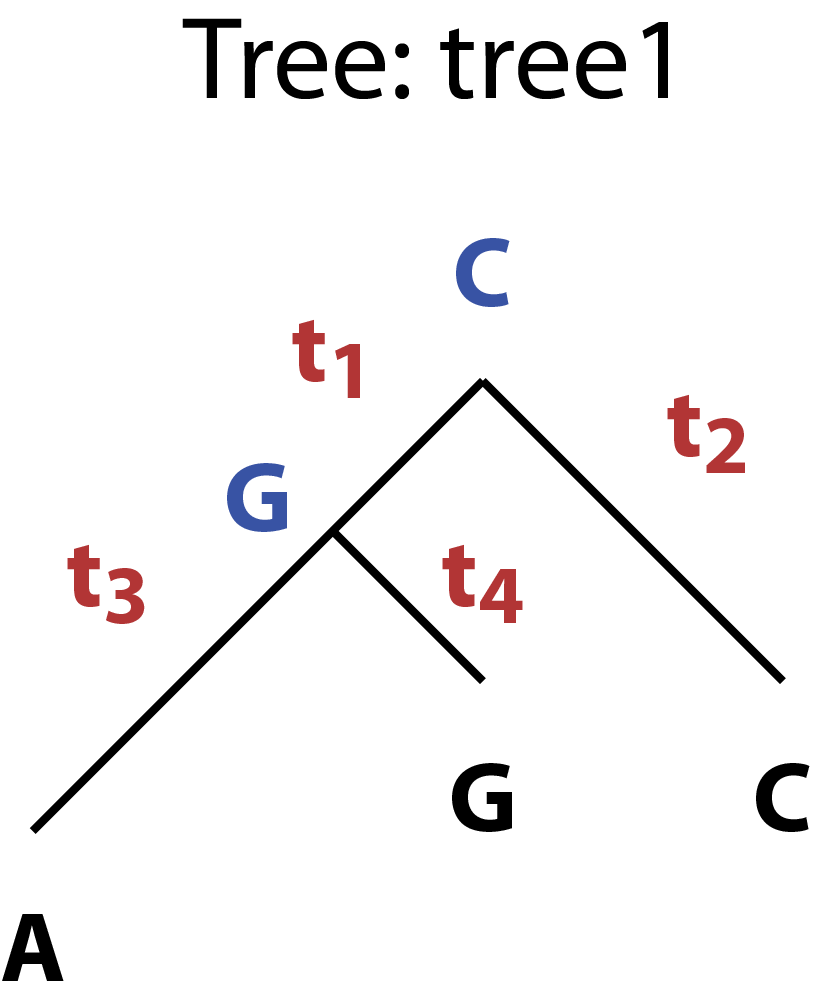
\includegraphics[width=0.2 \textwidth]{fig09/ml_tree.png}
      \caption{Two dice - a fair die and a die with three 6’s}
\end{figure}
 
Likelihood: $L(T=tree1|D ) = P(D|T=tree1 )=P_{CG}(t{1})P_{CC}(t_{2})P_{GA}(t_{3})P_{GG}(t_{4})$

%
% Log-likelihood
%
\subsubsection*{Log-likelihood}
\begin{itemize}
\item Logarithm is a monotonically increasing function 
\item $\log⁡(ab)=\log⁡(a)+\log⁡(b)$
\end{itemize}

%
% Time complexity of tree search
%
\subsubsection*{Time complexity of tree search}
Since it needs to search all possible trees, both the maximum parsimony and the maximum likelihood methods are NP hard problems. 
\begin{itemize}
\item Exhaustive search: up to 8-10 sequences
\item Branch and bound or pruning: up to 15-20 sequences
\item Heuristics: 100+ sequences
\end{itemize}

\bigskip 

%\end{document}


\end{document}
